
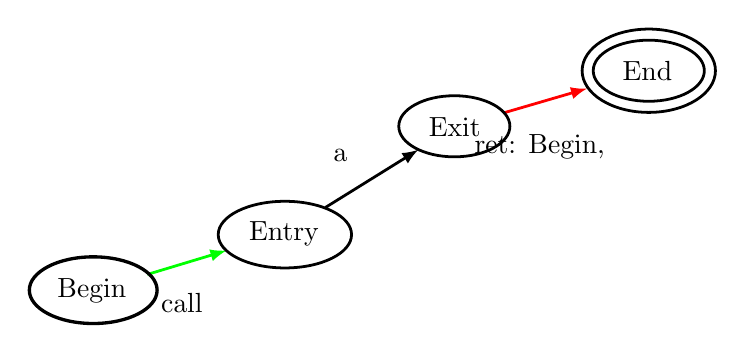
\begin{tikzpicture}[>=latex,line join=bevel,]
  \pgfsetlinewidth{1bp}
%%
\pgfsetcolor{black}
  % Edge: Exit -> End
  \pgfsetcolor{red}
  \draw [->] (172.65bp,77.794bp) .. controls (178.8bp,79.589bp) and (185.91bp,81.665bp)  .. (202.79bp,86.594bp);
  \definecolor{strokecol}{rgb}{0.0,0.0,0.0};
  \pgfsetstrokecolor{strokecol}
  \draw (185.75bp,65.744bp) node {ret: Begin, };
  % Edge: Entry -> Exit
  \draw [->] (108.54bp,43.739bp) .. controls (115.98bp,48.358bp) and (125.12bp,54.036bp)  .. (142.07bp,64.561bp);
  \draw (113.94bp,62.437bp) node {a};
  % Edge: Begin -> Entry
  \pgfsetcolor{green}
  \draw [->] (44.502bp,19.669bp) .. controls (50.366bp,21.438bp) and (56.915bp,23.413bp)  .. (72.976bp,28.258bp);
  \definecolor{strokecol}{rgb}{0.0,0.0,0.0};
  \pgfsetstrokecolor{strokecol}
  \draw (56.887bp,9.5bp) node {call};
  % Node: Entry
\begin{scope}
  \definecolor{strokecol}{rgb}{0.0,0.0,0.0};
  \pgfsetstrokecolor{strokecol}
  \draw (94bp,34bp) ellipse (24bp and 12bp);
  \draw (93.654bp,34.495bp) node {Entry};
\end{scope}
  % Node: Begin
\begin{scope}
  \definecolor{strokecol}{rgb}{0.0,0.0,0.0};
  \pgfsetstrokecolor{strokecol}
  \draw [very thick] (25bp,14bp) ellipse (23bp and 12bp);
  \draw (24.5bp,13.636bp) node {Begin};
\end{scope}
  % Node: End
\begin{scope}
  \definecolor{strokecol}{rgb}{0.0,0.0,0.0};
  \pgfsetstrokecolor{strokecol}
  \draw (225bp,93bp) ellipse (20bp and 11bp);
  \draw (225bp,93bp) ellipse (24bp and 15bp);
  \draw (224.5bp,92.936bp) node {End};
\end{scope}
  % Node: Exit
\begin{scope}
  \definecolor{strokecol}{rgb}{0.0,0.0,0.0};
  \pgfsetstrokecolor{strokecol}
  \draw (155bp,73bp) ellipse (20bp and 11bp);
  \draw (155.15bp,72.683bp) node {Exit};
\end{scope}
%
\end{tikzpicture}
